\subsection{Disparity Algorithm}
After verifying that the camera interface was functional, a large portion of time was spent implementing a disparity algorithm that would allow for the extraction of 3D depth information from stereo image data. This algorithm was first implemented in \textsc{Matlab}, and was then transferred to programmable logic after the algorithm was verified working. 
\subsubsection{Camera Rectification}
\begin{figure}[H]
	\centerline{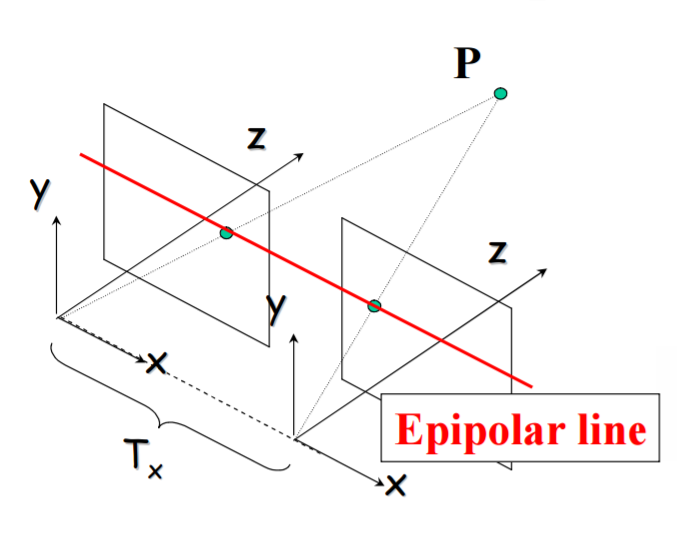
\includegraphics[width=0.75\textwidth]{epipolarLines.PNG}}
	\caption{Horizontal Epipolar Lines \cite{collins}}
	\label{epipolarLines}
\end{figure}

\subsubsection{Sum of Absolute Differences}
The method used in our disparity algorithm implementation
\begin{figure}[H]
	\centerline{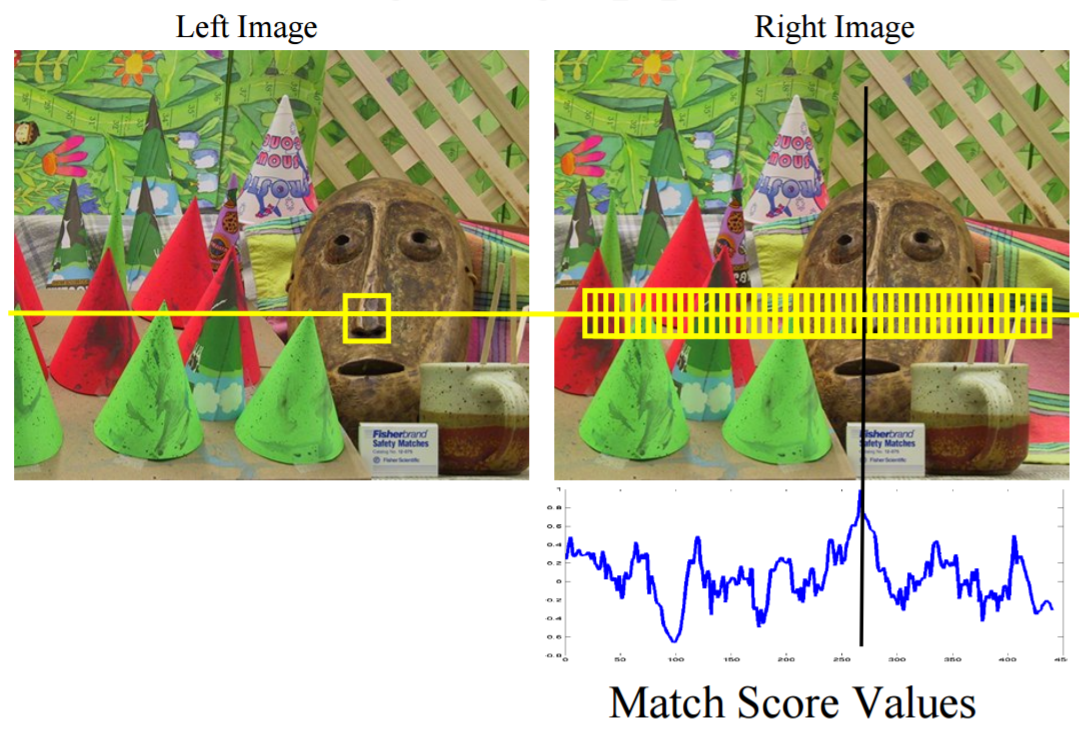
\includegraphics[width=0.75\textwidth]{blockMatching.PNG}}
	\caption{Block Matching Overview \cite{collins}}
	\label{blockMatching}
\end{figure}
\begin{figure}[H]
	\centerline{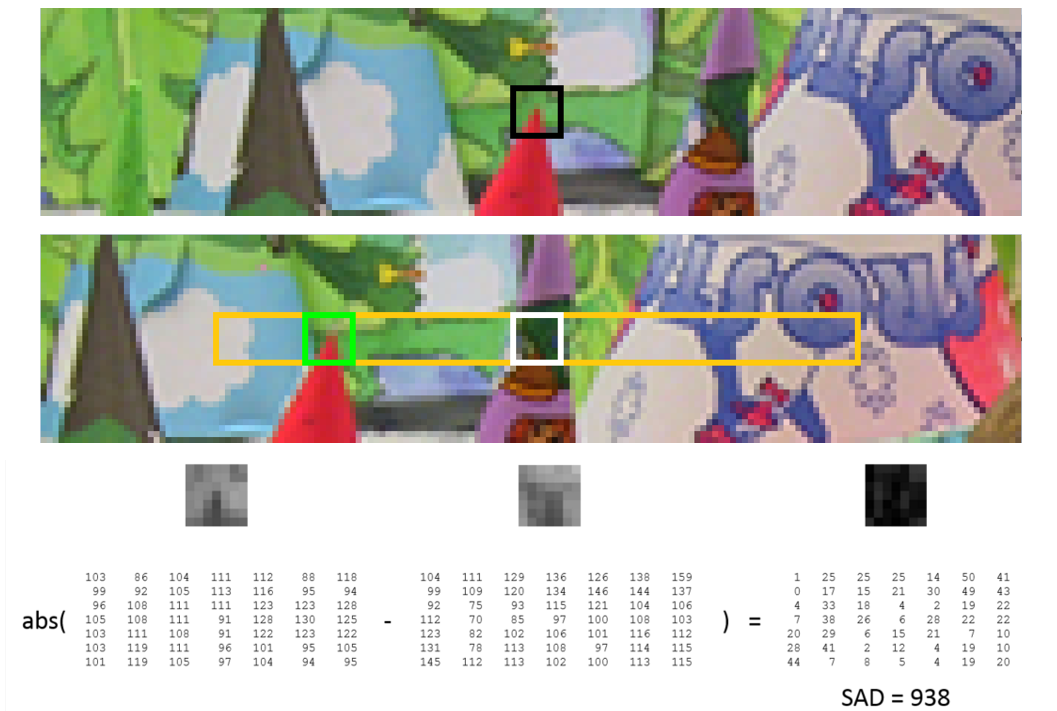
\includegraphics[width=0.75\textwidth]{SAD.PNG}}
	\caption{Sum of Absolute Differences \cite{mccormick}}
	\label{SAD}
\end{figure}

\subsubsection{Test Implementation}
\subsubsection{Final Implementation}